\section{Resultat}
\subsection{System 1}
Den analytiska lösningen för system 1 är
\begin{equation*}
    \begin{cases}
        x=\frac{27}{46}\cos(\frac{\sqrt{53}x}{5})+\sqrt{53}\sin(\frac{-\sqrt{53}x}{5})+\\
        \qquad\frac{-19}{46\sqrt{53}}(\sqrt{53}\cos(\frac{\sqrt{53}x}{5})+27\sin(\frac{-\sqrt{53}x}{5})\\
        \\[-7.5pt]
        y=\cos(\frac{\sqrt{53}}{5}t)+\frac{-19}{\sqrt{53}}\sin(\frac{-\sqrt{53}}{5}t)
    \end{cases}
\end{equation*}. En graf över olika steglängder och de associerade felen finnes i figur \ref{fig:diagram_sys_1_errors}.

\begin{figure}[h!]
    \centering
    % Automatically generated code. github.com/ohman-emil/GA
\begin{tikzpicture}
\definecolor{clr0}{RGB}{0, 114, 189}
\definecolor{clr1}{RGB}{217, 83, 25}
\definecolor{clr2}{RGB}{237, 177, 32}
\definecolor{clr3}{RGB}{126, 47, 142}
\definecolor{clr4}{RGB}{119, 172, 48}
\definecolor{clr5}{RGB}{77, 190, 238}
\definecolor{clr6}{RGB}{162, 20, 47}
\definecolor{clr7}{RGB}{120, 120, 120}
\begin{axis}[xmode=log,ymode=log,xlabel=Steglängd,ylabel=Avvikelse,width=\textwidth,height=0.6\textwidth,grid=both,minor grid style={draw=gray!33},major grid style={draw=gray},legend pos=south east,legend columns=2,legend style={column sep=1.5ex},]
\addplot[line width=1pt,mark=*,color=clr0] table {
0.05 1.6750755792762828
0.025 1.6836670243033418
0.0125 1.6438159414201832
0.00625 1.4104628232068364
0.003125 1.0016101885757394
0.0015625 0.6110836745847075
0.00078125 0.3395972996811829
0.000390625 0.17929090939529457
};
\addlegendentry{\hspace{{-1.25ex}}Euler 1}
\addplot[line width=1pt,mark=*,color=clr1] table {
0.05 2.5385976912679484
0.025 2.5788057118256185
0.0125 2.5327536079228596
0.00625 2.177537353746312
0.003125 1.5449812852953864
0.0015625 0.9412778612469512
0.00078125 0.522562409122171
0.000390625 0.27572173340265005
};
\addlegendentry{\hspace{{-1.25ex}}Euler 2}
\addplot[line width=1pt,mark=*,color=clr2] table {
0.05 0.009094604916475069
0.025 0.0016945605347229442
0.0125 0.000344297433158669
0.00625 7.571383342752647e-05
0.003125 1.760560197339167e-05
0.0015625 4.23430494400634e-06
0.00078125 1.0375805974405239e-06
0.000390625 2.567638994754873e-07
};
\addlegendentry{\hspace{{-1.25ex}}Heun 1}
\addplot[line width=1pt,mark=*,color=clr3] table {
0.05 0.03271401808365315
0.025 0.0073081808942934146
0.0125 0.001706531440970327
0.00625 0.00041079809817334834
0.003125 0.00010067098463961699
0.0015625 2.491107442459395e-05
0.00078125 6.195489655524966e-06
0.000390625 1.5448252912442229e-06
};
\addlegendentry{\hspace{{-1.25ex}}Heun 2}
\end{axis}
\end{tikzpicture}
    \caption{Avvikelsen i system 1 för de olika funktionerna.}
    \label{fig:diagram_sys_1_errors}
\end{figure}

\subsection{System 2}
Den analytiska lösningen för system 2 är
\begin{equation*}
    \begin{cases}
        x=(\frac{-36}{71}\cos(\frac{\sqrt{31}t}{5})-\frac{2\sqrt{31}}{71}\sin(\frac{\sqrt{31}t}{5}))+\\
        \qquad \frac{107}{142\sqrt{31}}(2\sqrt{31}\cos(\frac{\sqrt{31}t}{5})-36\sin(\frac{\sqrt{31}t}{5}))\\
        \\[-7.5pt]
        y=\cos({\frac{\sqrt{31}t}{5}})+\frac{107}{2\sqrt{31}}\sin(\frac{\sqrt{31}t}{5})
    \end{cases}
\end{equation*}. En graf över olika steglängder och de associerade felen finnes i figur \ref{fig:diagram_sys_2_errors}.

\begin{figure}[h!]
    \centering
    % Automatically generated code. github.com/ohman-emil/GA
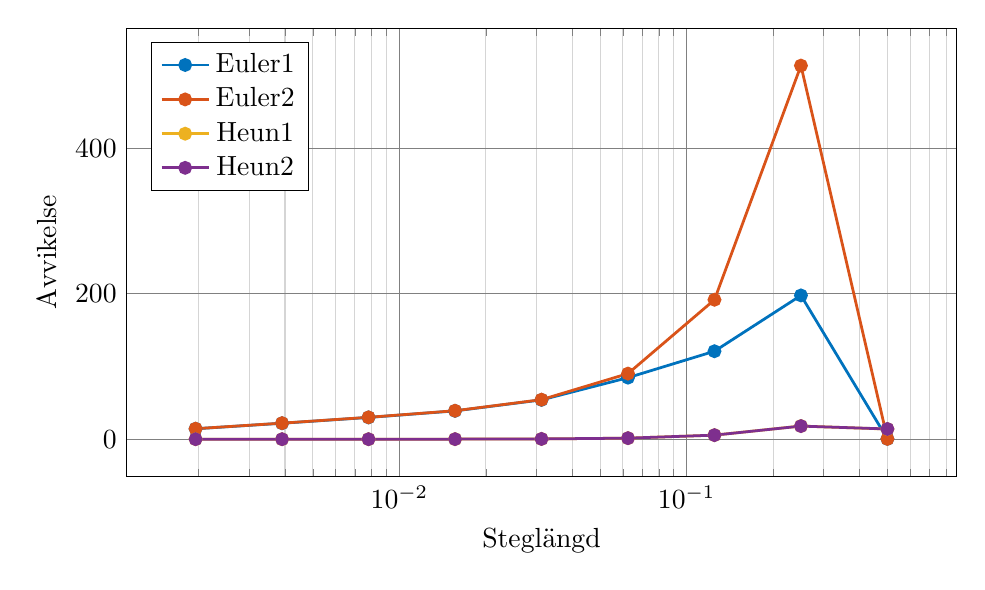
\begin{tikzpicture}
\definecolor{clr0}{RGB}{0, 114, 189}
\definecolor{clr1}{RGB}{217, 83, 25}
\definecolor{clr2}{RGB}{237, 177, 32}
\definecolor{clr3}{RGB}{126, 47, 142}
\definecolor{clr4}{RGB}{119, 172, 48}
\definecolor{clr5}{RGB}{77, 190, 238}
\definecolor{clr6}{RGB}{162, 20, 47}
\begin{axis}[xmode=log,xlabel=Steglängd,ylabel=Avvikelse,width=\textwidth,height=0.6\textwidth,grid=both,minor grid style={draw=gray!33},major grid style={draw=gray},legend pos=north west,]
\addplot[line width=1pt,mark=*,color=clr0,] table {
0.5 0.4211841737516414
0.25 197.723466709846
0.125 120.9725104910133
0.0625 84.6140176455516
0.03125 54.04753221969218
0.015625 38.92348052184204
0.0078125 29.926022452201458
0.00390625 21.933766067473083
0.001953125 14.339121755351952
};
\addlegendentry{Euler1}
\addplot[line width=1pt,mark=*,color=clr1,] table {
0.5 0.4211841737516414
0.25 513.7927940776342
0.125 191.74430670981843
0.0625 90.20697109755207
0.03125 54.37243071179283
0.015625 39.135490642700624
0.0078125 30.093036456717865
0.00390625 22.07127080595174
0.001953125 14.440463426487897
};
\addlegendentry{Euler2}
\addplot[line width=1pt,mark=*,color=clr2,] table {
0.5 13.898052418978153
0.25 18.098085624432596
0.125 5.592932249128091
0.0625 1.431875342118559
0.03125 0.3591328746325572
0.015625 0.0898260081759242
0.0078125 0.022458662866122765
0.00390625 0.005614835325139018
0.001953125 0.0014037250424195965
};
\addlegendentry{Heun1}
\addplot[line width=1pt,mark=*,color=clr3,] table {
0.5 14.06232025683895
0.25 18.015541487274373
0.125 5.570913124360444
0.0625 1.4282095972367266
0.03125 0.3579875087879995
0.015625 0.08952612691348509
0.0078125 0.02238134961045489
0.00390625 0.005595180830375101
0.001953125 0.0013987692610757903
};
\addlegendentry{Heun2}
\end{axis}
\end{tikzpicture}
    \caption{Avvikelsen i system 2 för de olika funktionerna.}
    \label{fig:diagram_sys_2_errors}
\end{figure}

\subsection{System 3}
Den analytiska lösningen för system 3 är
\begin{equation*}
    \begin{cases}
        x=(\frac{78}{73}\cos(\frac{\sqrt{231}t}{5})-\frac{2\sqrt{231}}{73}\sin(\frac{\sqrt{231}t}{5})-\\
        \qquad \frac{5}{2\sqrt{231}}(\frac{2\sqrt{231}}{73}\cos(\frac{\sqrt{231}t}{5})-\frac{78}{73}\sin(\frac{\sqrt{231}t}{5}))\\
        \\[-7.5pt]
        y=\cos({\frac{\sqrt{231}t}{5}})-\frac{5}{2\sqrt{231}}\sin(\frac{\sqrt{231}t}{5})
    \end{cases}
\end{equation*}. En graf över olika steglängder och de associerade felen finnes i figur \ref{fig:diagram_sys_3_errors}.

\begin{figure}[h!]
    \centering
    % Automatically generated code. github.com/ohman-emil/GA
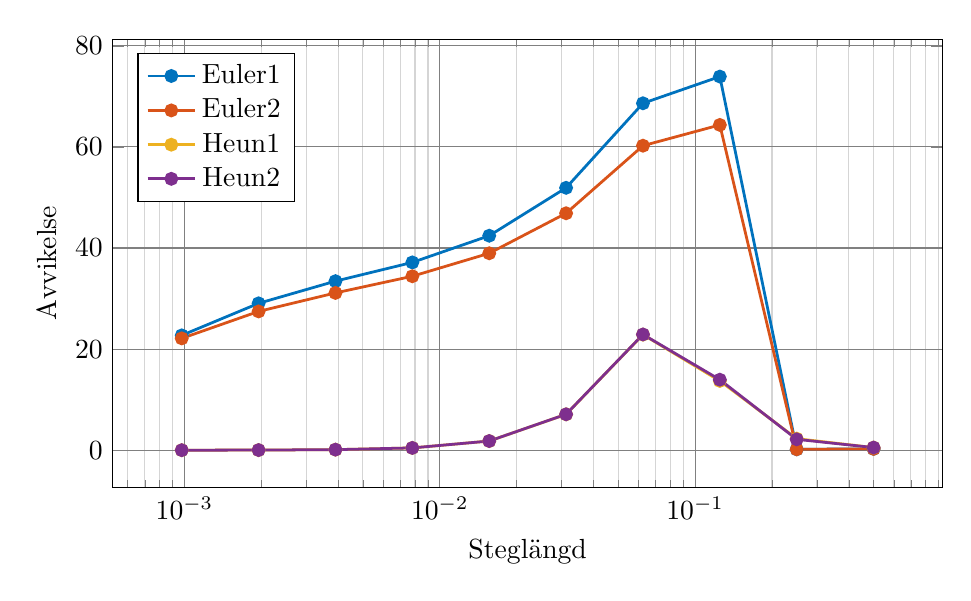
\begin{tikzpicture}
\definecolor{clr0}{RGB}{0, 114, 189}
\definecolor{clr1}{RGB}{217, 83, 25}
\definecolor{clr2}{RGB}{237, 177, 32}
\definecolor{clr3}{RGB}{126, 47, 142}
\definecolor{clr4}{RGB}{119, 172, 48}
\definecolor{clr5}{RGB}{77, 190, 238}
\definecolor{clr6}{RGB}{162, 20, 47}
\begin{axis}[xmode=log,xlabel=Steglängd,ylabel=Avvikelse,width=\textwidth,height=0.6\textwidth,grid=both,minor grid style={draw=gray!33},major grid style={draw=gray},legend pos=north west,]
\addplot[line width=1pt,mark=*,color=clr0,] table {
0.5 0.2662473304209822
0.25 0.18070600942864984
0.125 73.91361240845563
0.0625 68.63201070142117
0.03125 51.91003960891383
0.015625 42.4299501782937
0.0078125 37.15248327720794
0.00390625 33.4463208149152
0.001953125 29.05919618734267
0.0009765625 22.718232564896493
};
\addlegendentry{Euler1}
\addplot[line width=1pt,mark=*,color=clr1,] table {
0.5 0.2662473304209822
0.25 0.18070600942864984
0.125 64.34896419142808
0.0625 60.239000265502895
0.03125 46.873450255040154
0.015625 38.9580911165428
0.0078125 34.412417032816926
0.00390625 31.11668228946688
0.001953125 27.45928353877614
0.0009765625 22.125542532698013
};
\addlegendentry{Euler2}
\addplot[line width=1pt,mark=*,color=clr2,] table {
0.5 0.522467374124247
0.25 2.2869979323006766
0.125 13.705718766946177
0.0625 22.869157660406074
0.03125 7.097115981569413
0.015625 1.815455866671304
0.0078125 0.45510968308561073
0.00390625 0.11381675981706915
0.001953125 0.028455476540583214
0.0009765625 0.007113906572758029
};
\addlegendentry{Heun1}
\addplot[line width=1pt,mark=*,color=clr3,] table {
0.5 0.525541182854665
0.25 2.153062972680837
0.125 13.948129330495066
0.0625 22.900233510293006
0.03125 7.108208143391555
0.015625 1.8168893112692335
0.0078125 0.45548805200232323
0.00390625 0.11391470537442648
0.001953125 0.028480674908483408
0.0009765625 0.00712032049348493
};
\addlegendentry{Heun2}
\end{axis}
\end{tikzpicture}
    \caption{Avvikelsen i system 3 för de olika funktionerna.}
    \label{fig:diagram_sys_3_errors}
\end{figure}

\subsection{System 4}
Den analytiska lösningen för system 4 är
\begin{equation*}
    \begin{cases}
        x=(\frac{20}{26}\cos(\frac{\sqrt{\frac{1}{2}203}t}{5})+\frac{\sqrt{406}}{26}\sin(\frac{\sqrt{\frac{1}{2}203}t}{5}))-\\
        \qquad \frac{6}{\sqrt{406}}(\frac{-\sqrt{406}}{26}\cos(\frac{\sqrt{\frac{1}{2}203}t}{5})-\frac{20}{26}\sin(\frac{\sqrt{\frac{1}{2}203}t}{5}))\\
        \\[-7.5pt]
        y=\cos({\frac{\sqrt{\frac{1}{2}203}t}{5}})+\frac{107}{2\sqrt{31}}\sin(\frac{\sqrt{\frac{1}{2}203}t}{5})
    \end{cases}
\end{equation*}. En graf över olika steglängder och de associerade felen finnes i figur \ref{fig:diagram_sys_4_errors}.

\begin{figure}[h!]
    \centering
    % Automatically generated code. github.com/ohman-emil/GA
\begin{tikzpicture}
\definecolor{clr0}{RGB}{0, 114, 189}
\definecolor{clr1}{RGB}{217, 83, 25}
\definecolor{clr2}{RGB}{237, 177, 32}
\definecolor{clr3}{RGB}{126, 47, 142}
\definecolor{clr4}{RGB}{119, 172, 48}
\definecolor{clr5}{RGB}{77, 190, 238}
\definecolor{clr6}{RGB}{162, 20, 47}
\definecolor{clr7}{RGB}{120, 120, 120}
\begin{axis}[xmode=log,ymode=log,xlabel=Steglängd,ylabel=Avvikelse,width=\textwidth,height=0.6\textwidth,grid=both,minor grid style={draw=gray!33},major grid style={draw=gray},legend pos=south east,legend columns=2,legend style={column sep=1.5ex},]
\addplot[line width=1pt,mark=*,color=clr0] table {
0.05 0.4078447222591455
0.025 0.3357051209457099
0.0125 0.2220457522484941
0.00625 0.12878090836144657
0.003125 0.069501117572981
0.0015625 0.03612328945795862
0.00078125 0.018417487668963783
0.000390625 0.009299338383892186
};
\addlegendentry{\hspace{{-1.25ex}}Euler 1}
\addplot[line width=1pt,mark=*,color=clr1] table {
0.05 0.8461904620475155
0.025 0.6304855912217
0.0125 0.3963181895759291
0.00625 0.2239451462132166
0.003125 0.1192756059016572
0.0015625 0.06158320420352448
0.00078125 0.031293772814663834
0.000390625 0.01577446337523747
};
\addlegendentry{\hspace{{-1.25ex}}Euler 2}
\addplot[line width=1pt,mark=*,color=clr2] table {
0.05 0.0719081338173948
0.025 0.01747030466198085
0.0125 0.004286688402155625
0.00625 0.0010601428549243952
0.003125 0.0002634952419886538
0.0015625 6.56747037979244e-05
0.00078125 1.6393367669564896e-05
0.000390625 4.09515179022879e-06
};
\addlegendentry{\hspace{{-1.25ex}}Heun 1}
\addplot[line width=1pt,mark=*,color=clr3] table {
0.05 0.027354572941000188
0.025 0.0057913512565404
0.0125 0.001289021320745709
0.00625 0.0003005449859478926
0.003125 7.230326690610411e-05
0.0015625 1.7714162785065213e-05
0.00078125 4.382860917973019e-06
0.000390625 1.0899756237581215e-06
};
\addlegendentry{\hspace{{-1.25ex}}Heun 2}
\end{axis}
\end{tikzpicture}
    \caption{Avvikelsen i system 4 för de olika funktionerna.}
    \label{fig:diagram_sys_4_errors}
\end{figure}

\subsection{System 5}
Den analytiska lösningen för system 5 är
\begin{equation*}
    \begin{cases}
        x=\frac{2416}{2371}(\frac{-23}{58}\cos(\frac{\sqrt{2371}t}{10})+\frac{\sqrt{2371}}{58}\sin(\frac{\sqrt{2371}t}{10}))-\\
        \qquad \frac{16}{\sqrt{2371}}(\frac{-\sqrt{2371}}{58}\cos(\frac{\sqrt{2371}t}{10})+\frac{23}{58}\sin(\frac{\sqrt{2371}t}{10}))+\frac{2675}{2371}\\
        \\[-7.5pt]
        y=\frac{2416}{2371}\cos(\frac{\sqrt{2371}t}{10})-\frac{+16}{\sqrt{2371}}\sin(\frac{\sqrt{2371}t}{10})-\frac{45}{2371}
    \end{cases}
\end{equation*}. Den motsvarande homogena differentialekvationen har lösningen 
\begin{equation*}
    \begin{cases}
        x=(\frac{-23}{58}\cos(\frac{\sqrt{2371}t}{10})+\frac{+\sqrt{2371}}{58}\sin(\frac{\sqrt{2371}t}{10}))-\\
        \qquad \frac{81}{\sqrt{2371}}(\frac{-\sqrt{2371}}{58}\cos(\frac{\sqrt{2371}t}{10})-\frac{-23}{58}\sin(\frac{\sqrt{2371}t}{10}))\\
        \\[-7.5pt]
        y=\cos(\frac{\sqrt{2371}t}{10})-\frac{81}{\sqrt{2371}}\sin(\frac{\sqrt{2371}t}{10})
    \end{cases}
\end{equation*}. En graf över olika steglängder och de associerade felen finnes i figur \ref{fig:diagram_sys_5_errors}.

\begin{figure}[h!]
    \centering

    \begin{subfigure}[h]{\textwidth}
        % Automatically generated code. github.com/ohman-emil/GA
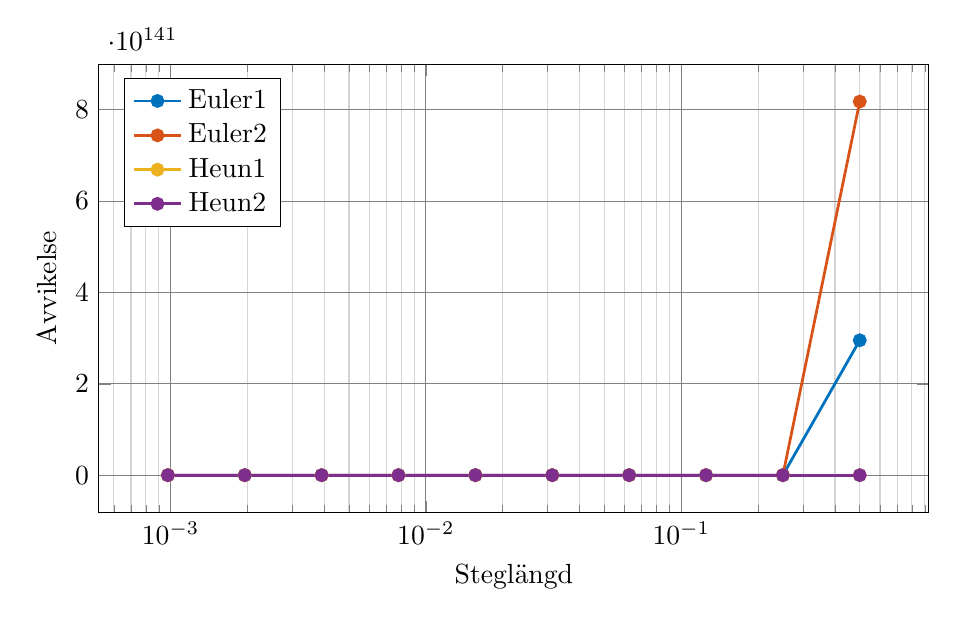
\begin{tikzpicture}
\definecolor{clr0}{RGB}{0, 114, 189}
\definecolor{clr1}{RGB}{217, 83, 25}
\definecolor{clr2}{RGB}{237, 177, 32}
\definecolor{clr3}{RGB}{126, 47, 142}
\definecolor{clr4}{RGB}{119, 172, 48}
\definecolor{clr5}{RGB}{77, 190, 238}
\definecolor{clr6}{RGB}{162, 20, 47}
\begin{axis}[xmode=log,xlabel=Steglängd,ylabel=Avvikelse,width=\textwidth,height=0.6\textwidth,grid=both,minor grid style={draw=gray!33},major grid style={draw=gray},legend pos=north west,]
\addplot[line width=1pt,mark=*,color=clr0,] table {
0.5 2.9524953778948422e+141
0.25 0.3167381985006317
0.125 0.30920293404134236
0.0625 0.2984074749081066
0.03125 0.27854828190558645
0.015625 0.24093298245438408
0.0078125 0.18221020057423795
0.00390625 0.11867892442296757
0.001953125 0.06897143705773831
0.0009765625 0.03736779649764003
};
\addlegendentry{Euler1}
\addplot[line width=1pt,mark=*,color=clr1,] table {
0.5 8.17817951512437e+141
0.25 0.32054295294251367
0.125 0.3122503019125455
0.0625 0.29944624330903635
0.03125 0.2785612200769082
0.015625 0.24044819211722657
0.0078125 0.18156804978113145
0.00390625 0.11813784462917352
0.001953125 0.06861487391059849
0.0009765625 0.03716220430862328
};
\addlegendentry{Euler2}
\addplot[line width=1pt,mark=*,color=clr2,] table {
0.5 8.893218770685648e+95
0.25 3.08312729811997e+35
0.125 16983.513903618365
0.0625 0.848390293494165
0.03125 0.29867887721661374
0.015625 0.07517023069112065
0.0078125 0.01872676993884599
0.00390625 0.004678531403668692
0.001953125 0.0011695389576915954
0.0009765625 0.0002923851122200028
};
\addlegendentry{Heun1}
\addplot[line width=1pt,mark=*,color=clr3,] table {
0.5 1.0912240774133727e+96
0.25 3.537597035239887e+35
0.125 16806.2827350711
0.0625 0.8473270588476569
0.03125 0.2986029778926087
0.015625 0.07500551189131384
0.0078125 0.018684370828993584
0.00390625 0.004667935904350018
0.001953125 0.001166890531406937
0.0009765625 0.00029172299759632874
};
\addlegendentry{Heun2}
\end{axis}
\end{tikzpicture}
        \caption{Homogen}
    \end{subfigure}
    %
    \vspace{1em}\newline
    %
    \begin{subfigure}[h]{\textwidth}
        % Automatically generated code. github.com/ohman-emil/GA
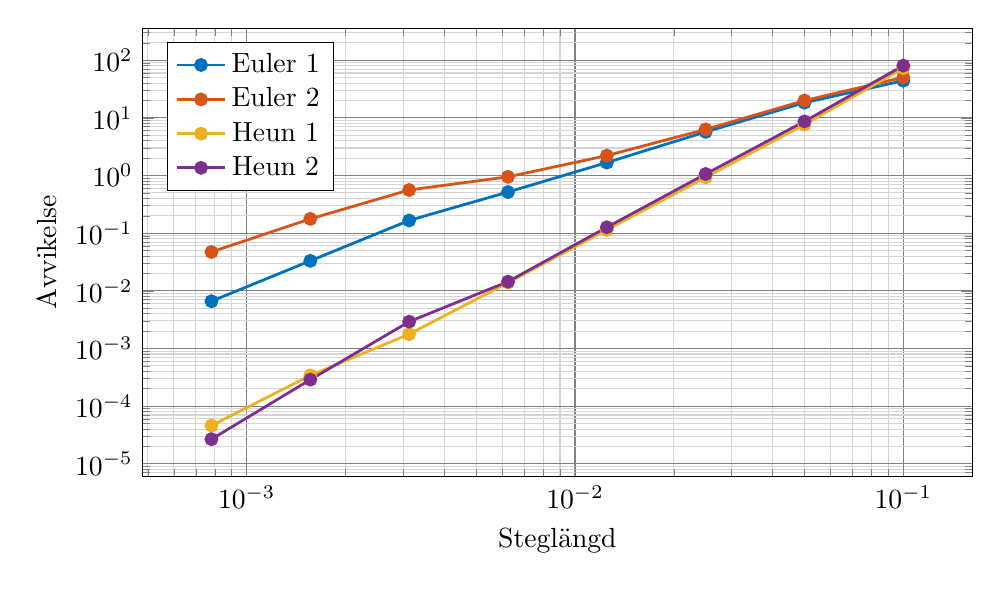
\begin{tikzpicture}
\definecolor{clr0}{RGB}{0, 114, 189}
\definecolor{clr1}{RGB}{217, 83, 25}
\definecolor{clr2}{RGB}{237, 177, 32}
\definecolor{clr3}{RGB}{126, 47, 142}
\definecolor{clr4}{RGB}{119, 172, 48}
\definecolor{clr5}{RGB}{77, 190, 238}
\definecolor{clr6}{RGB}{162, 20, 47}
\begin{axis}[xmode=log,ymode=log,xlabel=Steglängd,ylabel=Avvikelse,width=\textwidth,height=0.6\textwidth,grid=both,minor grid style={draw=gray!33},major grid style={draw=gray},legend pos=north west,]
\addplot[line width=1pt,mark=*,color=clr0] table {
0.1 44.05988947115482
0.05 18.294784015171874
0.025 5.696437609633072
0.0125 1.6744928679218927
0.00625 0.516186554058301
0.003125 0.16604067253281807
0.0015625 0.03309688797361421
0.00078125 0.006595852400765878
};
\addlegendentry{Euler 1}
\addplot[line width=1pt,mark=*,color=clr1] table {
0.1 50.316024645513856
0.05 19.94655563413939
0.025 6.296843297397823
0.0125 2.2127468346309094
0.00625 0.9472320651705217
0.003125 0.5602436166051301
0.0015625 0.1769965280384489
0.00078125 0.04714636660480531
};
\addlegendentry{Euler 2}
\addplot[line width=1pt,mark=*,color=clr2] table {
0.1 72.83752332493279
0.05 7.6472384155992685
0.025 0.927862085117403
0.0125 0.1139163047277526
0.00625 0.013838886580395782
0.003125 0.001770302811697988
0.0015625 0.00034075311144121656
0.00078125 4.599289630324854e-05
};
\addlegendentry{Heun 1}
\addplot[line width=1pt,mark=*,color=clr3] table {
0.1 80.55766432255909
0.05 8.671884399174639
0.025 1.0614103975665081
0.0125 0.12647852784222768
0.00625 0.014429650936993561
0.003125 0.002913694353494641
0.0015625 0.0002874589344831202
0.00078125 2.6681944061413e-05
};
\addlegendentry{Heun 2}
\end{axis}
\end{tikzpicture}
        \caption{Inhomogen}
    \end{subfigure}

    \caption{Avvikelsen i system 5 för de olika funktionerna.}
    \label{fig:diagram_sys_5_errors}
\end{figure}

\subsection{System 6}
Den analytiska lösningen för system 6 är
\begin{equation*}
    \begin{cases}
        x=\frac{1194}{103}(\frac{-72}{55}\cos(\frac{\sqrt{\frac{1}{2}103}t}{5})+\frac{\sqrt{206}}{55}\sin(\frac{\sqrt{\frac{1}{2}103}t}{5}))-\\
        \qquad \frac{43\sqrt{206}}{103}(\frac{-\sqrt{206}}{55}\cos(\frac{\sqrt{\frac{1}{2}103}t}{5})+\frac{72}{55}\sin(\frac{\sqrt{\frac{1}{2}103}t}{5}))+\frac{1505}{103}\\
        \\[-7.5pt]
        y=\frac{1194}{103}\cos({\frac{\sqrt{\frac{1}{2}103}t}{5}})-\frac{43\sqrt{206}}{103}\sin(\frac{\sqrt{\frac{1}{2}103}t}{5})-\frac{1091}{103}
    \end{cases}
\end{equation*}. Den motsvarande homogena differentialekvationen har lösningen 
\begin{equation*}
    \begin{cases}
        x=(\frac{-72}{55}\cos(\frac{\sqrt{\frac{1}{2}103}t}{5})+\frac{\sqrt{206}}{55}\sin(\frac{\sqrt{\frac{1}{2}103}t}{5}))-\\
        \qquad \frac{127}{\sqrt{206}}(\frac{-\sqrt{206}}{55}\cos(\frac{\sqrt{\frac{1}{2}103}t}{5})+\frac{72}{55}\sin(\frac{\sqrt{\frac{1}{2}103}t}{5}))\\
        \\[-7.5pt]
        y=\cos({\frac{\sqrt{\frac{1}{2}103}t}{5}})-\frac{127}{\sqrt{206}}\sin(\frac{\sqrt{\frac{1}{2}103}t}{5})
    \end{cases}
\end{equation*}. En graf över olika steglängder och de associerade felen finnes i figur \ref{fig:diagram_sys_6_errors}.

\begin{figure}[h!]
    \centering

    \begin{subfigure}[h]{\textwidth}
        % Automatically generated code. github.com/ohman-emil/GA
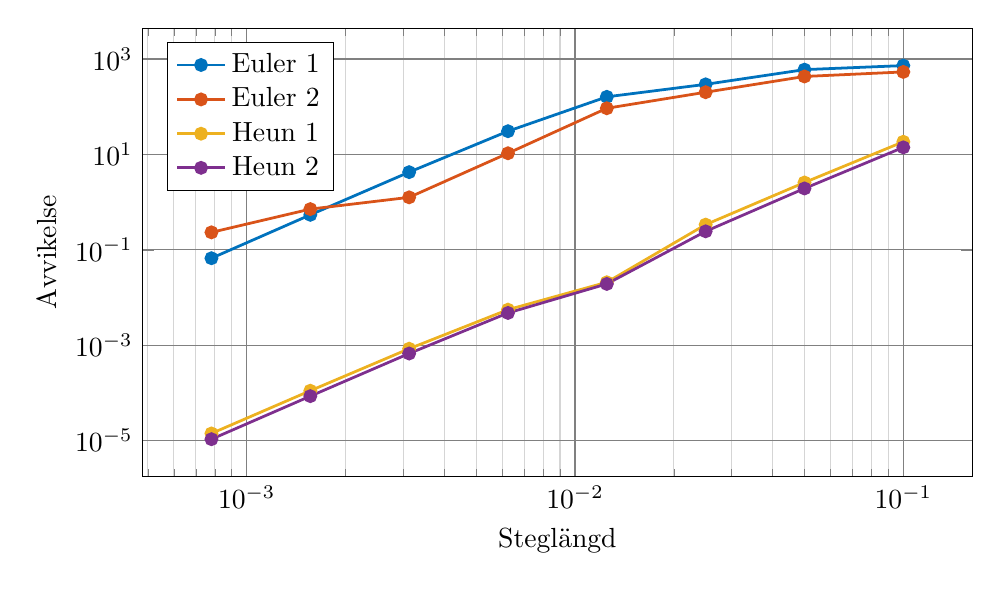
\begin{tikzpicture}
\definecolor{clr0}{RGB}{0, 114, 189}
\definecolor{clr1}{RGB}{217, 83, 25}
\definecolor{clr2}{RGB}{237, 177, 32}
\definecolor{clr3}{RGB}{126, 47, 142}
\definecolor{clr4}{RGB}{119, 172, 48}
\definecolor{clr5}{RGB}{77, 190, 238}
\definecolor{clr6}{RGB}{162, 20, 47}
\begin{axis}[xmode=log,ymode=log,xlabel=Steglängd,ylabel=Avvikelse,width=\textwidth,height=0.6\textwidth,grid=both,minor grid style={draw=gray!33},major grid style={draw=gray},legend pos=north west,]
\addplot[line width=1pt,mark=*,color=clr0] table {
0.1 728.782917316358
0.05 599.4770899575655
0.025 294.75437750751473
0.0125 161.23123894509473
0.00625 30.657014872267276
0.003125 4.246565083036572
0.0015625 0.5403589767551216
0.00078125 0.06654424815209636
};
\addlegendentry{Euler 1}
\addplot[line width=1pt,mark=*,color=clr1] table {
0.1 536.4730450691388
0.05 430.84864463375595
0.025 201.41440121215342
0.0125 92.80460552212948
0.00625 10.568622648295836
0.003125 1.2580098624521365
0.0015625 0.7129107481850188
0.00078125 0.2320796924746035
};
\addlegendentry{Euler 2}
\addplot[line width=1pt,mark=*,color=clr2] table {
0.1 18.405138906106114
0.05 2.574510634306033
0.025 0.3370121731740936
0.0125 0.02082705606944857
0.00625 0.005548458039600135
0.003125 0.0008416045323991206
0.0015625 0.00011075852439046407
0.00078125 1.4065161648924018e-05
};
\addlegendentry{Heun 1}
\addplot[line width=1pt,mark=*,color=clr3] table {
0.1 14.053409418292846
0.05 1.9315723391082273
0.025 0.2436781363996786
0.0125 0.0192245405200121
0.00625 0.004732733694065794
0.003125 0.0006677625851893854
0.0015625 8.521974713803643e-05
0.00078125 1.066287282832333e-05
};
\addlegendentry{Heun 2}
\end{axis}
\end{tikzpicture}
        \caption{Homogen}
    \end{subfigure}
    %
    \vspace{1em}\newline
    %
    \begin{subfigure}[h]{\textwidth}
        % Automatically generated code. github.com/ohman-emil/GA
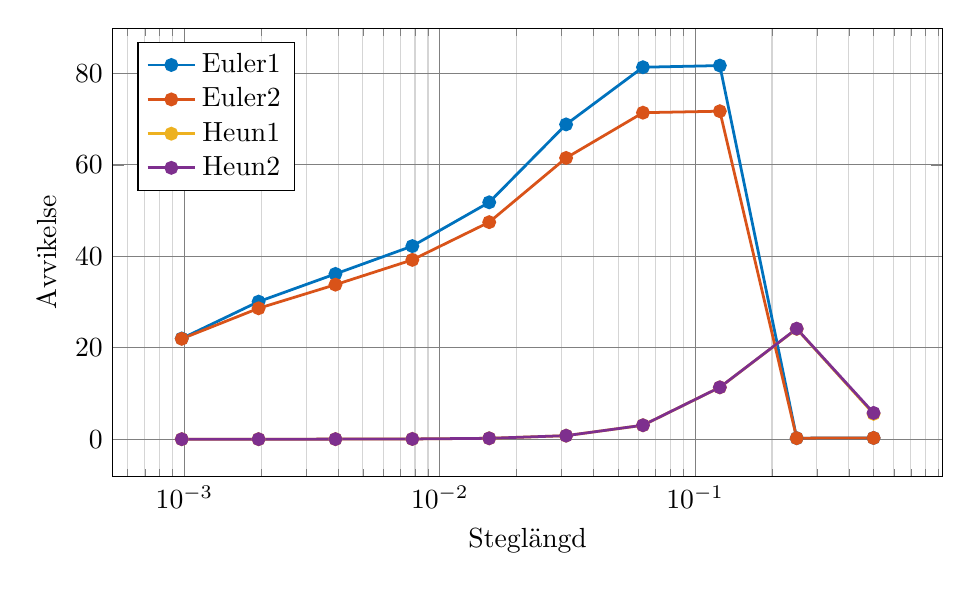
\begin{tikzpicture}
\definecolor{clr0}{RGB}{0, 114, 189}
\definecolor{clr1}{RGB}{217, 83, 25}
\definecolor{clr2}{RGB}{237, 177, 32}
\definecolor{clr3}{RGB}{126, 47, 142}
\definecolor{clr4}{RGB}{119, 172, 48}
\definecolor{clr5}{RGB}{77, 190, 238}
\definecolor{clr6}{RGB}{162, 20, 47}
\begin{axis}[xmode=log,xlabel=Steglängd,ylabel=Avvikelse,width=\textwidth,height=0.6\textwidth,grid=both,minor grid style={draw=gray!33},major grid style={draw=gray},legend pos=north west,]
\addplot[line width=1pt,mark=*,color=clr0,] table {
0.5 0.2718595058731115
0.25 0.21897879015386532
0.125 81.6990867577343
0.0625 81.34058285019368
0.03125 68.83245161115607
0.015625 51.80079885284301
0.0078125 42.2262708199145
0.00390625 36.14255148248802
0.001953125 30.079197166294982
0.0009765625 22.016448242199168
};
\addlegendentry{Euler1}
\addplot[line width=1pt,mark=*,color=clr1,] table {
0.5 0.2718595058731115
0.25 0.21897879015386534
0.125 71.72195798087068
0.0625 71.39818150668398
0.03125 61.501168763321644
0.015625 47.45945795447348
0.0078125 39.21277336072139
0.00390625 33.78950199841171
0.001953125 28.621668227506028
0.0009765625 21.95171493647992
};
\addlegendentry{Euler2}
\addplot[line width=1pt,mark=*,color=clr2,] table {
0.5 5.5363519676886135
0.25 24.115543956046874
0.125 11.334094259611026
0.0625 3.044662905772556
0.03125 0.7673487294692585
0.015625 0.19206174098955892
0.0078125 0.04802346395089087
0.00390625 0.012006259029565714
0.001953125 0.0030015897891863662
0.0009765625 0.0007503995477734864
};
\addlegendentry{Heun1}
\addplot[line width=1pt,mark=*,color=clr3,] table {
0.5 5.7395051886914255
0.25 24.16504274859443
0.125 11.34224346193682
0.0625 3.0485497070621133
0.03125 0.7680351728905486
0.015625 0.1922326149480055
0.0078125 0.04806964377137049
0.00390625 0.012018212328934502
0.001953125 0.0030046328905370275
0.0009765625 0.0007511673215743797
};
\addlegendentry{Heun2}
\end{axis}
\end{tikzpicture}
        \caption{Inhomogen}
    \end{subfigure}

    \caption{Avvikelsen i system 6 för de olika funktionerna.}
    \label{fig:diagram_sys_6_errors}
\end{figure}

\subsection{System 7}
Den analytiska lösningen för system 7 är
\begin{equation*}
    \begin{cases}
        x=\frac{739}{13}(\frac{-38}{35}\cos(\frac{\sqrt{26t}}{5})+\frac{\sqrt{26}}{35}\sin(\frac{\sqrt{26t}}{5}))-\\
        \qquad \frac{73}{\sqrt{26}}(\frac{\sqrt{26}}{35}\cos(\frac{\sqrt{26t}}{5})-\frac{38}{35}\sin(\frac{\sqrt{26t}}{5}))+\frac{1585}{26}\\
        \\[-7.5pt]
        y=\frac{739}{13}\cos(\frac{\sqrt{26t}}{5})+\frac{38}{35}\sin(\frac{\sqrt{26t}}{5})-\frac{726}{13}
    \end{cases}
\end{equation*}. Den motsvarande homogena differentialekvationen har lösningen 
\begin{equation*}
    \begin{cases}
        x=(\frac{-38}{35}\cos(\frac{\sqrt{26t}}{5})+\frac{\sqrt{26}}{35}\sin(\frac{\sqrt{26t}}{5}))-\\
        \qquad \frac{73}{\sqrt{26}}(\frac{\sqrt{26}}{35}\cos(\frac{\sqrt{26t}}{5})-\frac{38}{35}\sin(\frac{\sqrt{26t}}{5}))\\
        \\[-7.5pt]
        y=\cos(\frac{\sqrt{26t}}{5})+\frac{38}{35}\sin(\frac{\sqrt{26t}}{5})
    \end{cases}
\end{equation*}. En graf över olika steglängder och de associerade felen finnes i figur \ref{fig:diagram_sys_7_errors}.

\begin{figure}[h!]
    \centering

    \begin{subfigure}[h]{\textwidth}
        % Automatically generated code. github.com/ohman-emil/GA
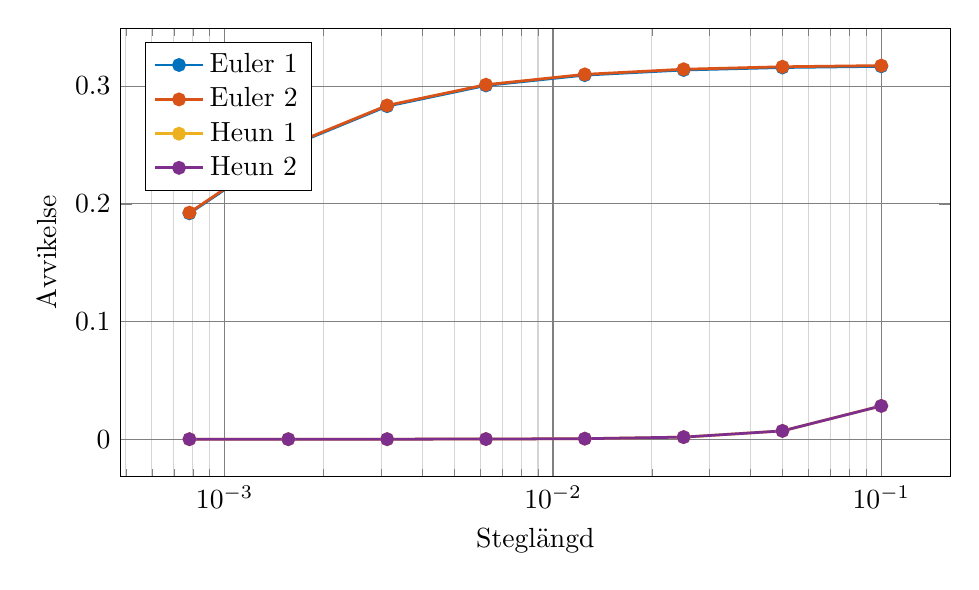
\begin{tikzpicture}
\definecolor{clr0}{RGB}{0, 114, 189}
\definecolor{clr1}{RGB}{217, 83, 25}
\definecolor{clr2}{RGB}{237, 177, 32}
\definecolor{clr3}{RGB}{126, 47, 142}
\definecolor{clr4}{RGB}{119, 172, 48}
\definecolor{clr5}{RGB}{77, 190, 238}
\definecolor{clr6}{RGB}{162, 20, 47}
\begin{axis}[xmode=log,xlabel=Steglängd,ylabel=Avvikelse,width=\textwidth,height=0.6\textwidth,grid=both,minor grid style={draw=gray!33},major grid style={draw=gray},legend pos=north west,]
\addplot[line width=1pt,mark=*,color=clr0] table {
0.1 0.31676231592572773
0.05 0.31578008832428295
0.025 0.3136684638238963
0.0125 0.3093129715340761
0.00625 0.30052401931498895
0.003125 0.2829072755968697
0.0015625 0.24841277979891796
0.00078125 0.19189258220425218
};
\addlegendentry{Euler 1}
\addplot[line width=1pt,mark=*,color=clr1] table {
0.1 0.31740945676890464
0.05 0.31641480765971397
0.025 0.3143034586041348
0.0125 0.30995393680154615
0.00625 0.3011691491395354
0.003125 0.2835551590138743
0.0015625 0.24905541419273192
0.00078125 0.19247525736873816
};
\addlegendentry{Euler 2}
\addplot[line width=1pt,mark=*,color=clr2] table {
0.1 0.028308601158391872
0.05 0.007058474786027166
0.025 0.0017639626045420902
0.0125 0.00044095351724727545
0.00625 0.00011023421586701235
0.003125 2.755799403495263e-05
0.0015625 6.889422499156318e-06
0.00078125 1.7223456750437312e-06
};
\addlegendentry{Heun 1}
\addplot[line width=1pt,mark=*,color=clr3] table {
0.1 0.028253631345154115
0.05 0.0070446301188025855
0.025 0.0017603950374059723
0.0125 0.0004400413329507993
0.00625 0.00011000310721516806
0.003125 2.7499802840691933e-05
0.0015625 6.874820777759947e-06
0.00078125 1.7186884252195757e-06
};
\addlegendentry{Heun 2}
\end{axis}
\end{tikzpicture}
        \caption{Homogen}
    \end{subfigure}
    %
    \vspace{1em}\newline
    %
    \begin{subfigure}[h]{\textwidth}
        % Automatically generated code. github.com/ohman-emil/GA
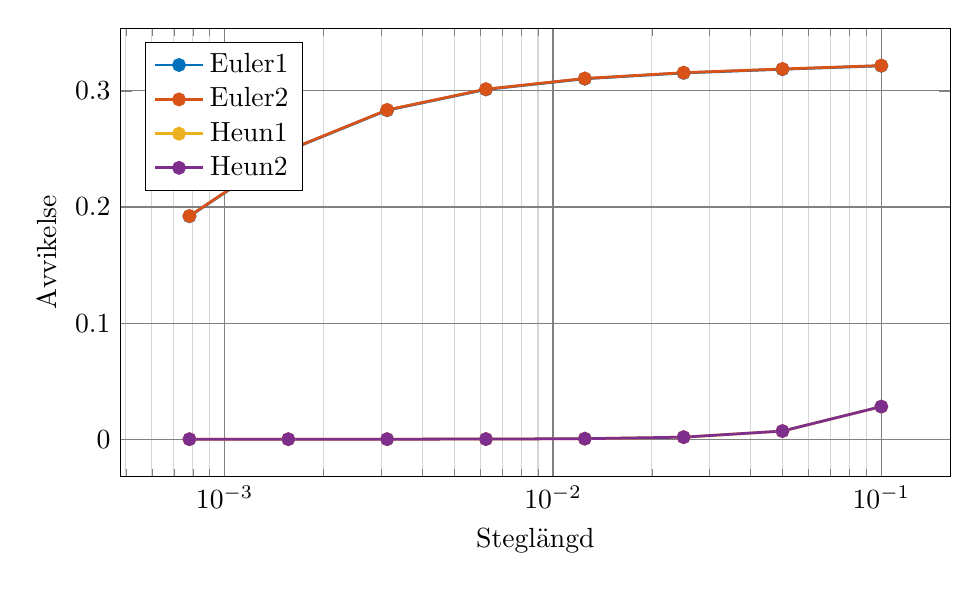
\begin{tikzpicture}
\definecolor{clr0}{RGB}{0, 114, 189}
\definecolor{clr1}{RGB}{217, 83, 25}
\definecolor{clr2}{RGB}{237, 177, 32}
\definecolor{clr3}{RGB}{126, 47, 142}
\definecolor{clr4}{RGB}{119, 172, 48}
\definecolor{clr5}{RGB}{77, 190, 238}
\definecolor{clr6}{RGB}{162, 20, 47}
\begin{axis}[xmode=log,xlabel=Steglängd,ylabel=Avvikelse,width=\textwidth,height=0.6\textwidth,grid=both,minor grid style={draw=gray!33},major grid style={draw=gray},legend pos=north west,]
\addplot[line width=1pt,mark=*,color=clr0,] table {
0.1 0.3216494459631003
0.05 0.3186894419072372
0.025 0.3155010969579957
0.0125 0.31049018416633123
0.00625 0.3012748590142731
0.003125 0.28338033592678913
0.0015625 0.24870288610680347
0.00078125 0.19205471318320733
};
\addlegendentry{Euler1}
\addplot[line width=1pt,mark=*,color=clr1,] table {
0.1 0.32182413148025785
0.05 0.3188929312540557
0.025 0.31571520059551966
0.0125 0.31071411312749964
0.00625 0.3015083792157432
0.003125 0.2836216187385052
0.0015625 0.24894602478257977
0.00078125 0.19227553744928286
};
\addlegendentry{Euler2}
\addplot[line width=1pt,mark=*,color=clr2,] table {
0.1 0.02806777402191016
0.05 0.006998173827219515
0.025 0.0017494564488447339
0.0125 0.00043743784796757484
0.00625 0.00010937172693539481
0.003125 2.734459306542522e-05
0.0015625 6.836360888945041e-06
0.00078125 1.7091171581375127e-06
};
\addlegendentry{Heun1}
\addplot[line width=1pt,mark=*,color=clr3,] table {
0.1 0.028099570857876722
0.05 0.007005942549586446
0.025 0.0017514615598952226
0.0125 0.0004379469594839387
0.00625 0.00010950025374228245
0.003125 2.737688329134967e-05
0.0015625 6.844454521521976e-06
0.00078125 1.7111432057757987e-06
};
\addlegendentry{Heun2}
\end{axis}
\end{tikzpicture}
        \caption{Inhomogen}
    \end{subfigure}

    \caption{Avvikelsen i system 7 för de olika funktionerna.}
    \label{fig:diagram_sys_7_errors}
\end{figure}

\subsection{System 8}
Den analytiska lösningen för system 8 är
\begin{equation*}
    \begin{cases}
        x=\frac{14139}{3029}(\frac{69}{82}\cos(\frac{\sqrt{3029t}}{10})+\frac{\sqrt{3029}}{82}\sin(\frac{\sqrt{3029t}}{10}))-\\
        \qquad \frac{73}{\sqrt{3029}}(\frac{\sqrt{3029}}{82}\cos(\frac{\sqrt{3029t}}{10})+\frac{69}{82}\sin(\frac{\sqrt{3029t}}{10}))-\frac{11565}{3029}\\
        \\[-7.5pt]
        y=\frac{14139}{3029}\cos(\frac{\sqrt{3029t}}{10})-\frac{73}{\sqrt{3029}}\sin(\frac{\sqrt{3029t}}{10})-\frac{11110}{3029}
    \end{cases}
\end{equation*}. Den motsvarande homogena differentialekvationen har lösningen 
\begin{equation*}
    \begin{cases}
        x=(\frac{69}{82}\cos(\frac{\sqrt{3029t}}{10})+\frac{\sqrt{3029}}{82}\sin(\frac{\sqrt{3029t}}{10}))-\\
        \qquad \sqrt{\frac{13}{233}}(\frac{\sqrt{3029}}{82}\cos(\frac{\sqrt{3029t}}{10})+\frac{69}{82}\sin(\frac{\sqrt{3029t}}{10}))\\
        \\[-7.5pt]
        y=\cos(\frac{\sqrt{3029t}}{10})-\sqrt{\frac{13}{233}}\sin(\frac{\sqrt{3029t}}{10})
    \end{cases}
\end{equation*}. En graf över olika steglängder och de associerade felen finnes i figur \ref{fig:diagram_sys_8_errors}.

\begin{figure}[h!]
    \centering

    \begin{subfigure}[h]{\textwidth}
        % Automatically generated code. github.com/ohman-emil/GA
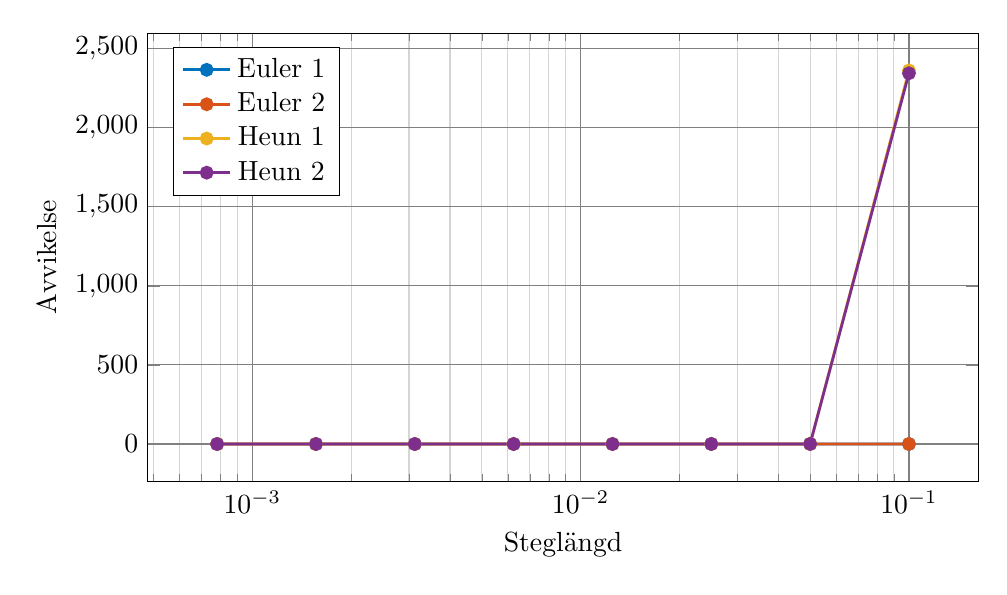
\begin{tikzpicture}
\definecolor{clr0}{RGB}{0, 114, 189}
\definecolor{clr1}{RGB}{217, 83, 25}
\definecolor{clr2}{RGB}{237, 177, 32}
\definecolor{clr3}{RGB}{126, 47, 142}
\definecolor{clr4}{RGB}{119, 172, 48}
\definecolor{clr5}{RGB}{77, 190, 238}
\definecolor{clr6}{RGB}{162, 20, 47}
\begin{axis}[xmode=log,xlabel=Steglängd,ylabel=Avvikelse,width=\textwidth,height=0.6\textwidth,grid=both,minor grid style={draw=gray!33},major grid style={draw=gray},legend pos=north west,]
\addplot[line width=1pt,mark=*,color=clr0] table {
0.1 0.3176957254115023
0.05 0.3163097677803269
0.025 0.3136035779533316
0.0125 0.3082240625312869
0.00625 0.2975042859040087
0.003125 0.27611939100865307
0.0015625 0.23535684066729462
0.00078125 0.1742758902863571
};
\addlegendentry{Euler 1}
\addplot[line width=1pt,mark=*,color=clr1] table {
0.1 0.31695930668221933
0.05 0.3156618004189254
0.025 0.3130023871459322
0.0125 0.30763900508396985
0.00625 0.2969365961926278
0.003125 0.2755650245978292
0.0015625 0.23482315802408757
0.00078125 0.17381760385785275
};
\addlegendentry{Euler 2}
\addplot[line width=1pt,mark=*,color=clr2] table {
0.1 2361.428659795269
0.05 0.7311125264279719
0.025 0.27559284618314306
0.0125 0.069271418290286
0.00625 0.017267182183972118
0.003125 0.004314366283655049
0.0015625 0.0010785191129063806
0.00078125 0.0002696299115164901
};
\addlegendentry{Heun 1}
\addplot[line width=1pt,mark=*,color=clr3] table {
0.1 2343.3971867183886
0.05 0.7316102910407278
0.025 0.27526200520084043
0.0125 0.06924857517318879
0.00625 0.017267411534630614
0.003125 0.004314668543116661
0.0015625 0.001078592697633467
0.00078125 0.00026964608135362155
};
\addlegendentry{Heun 2}
\end{axis}
\end{tikzpicture}
        \caption{Homogen}
    \end{subfigure}
    %
    \vspace{1em}\newline
    %
    \begin{subfigure}[h]{\textwidth}
        % Automatically generated code. github.com/ohman-emil/GA
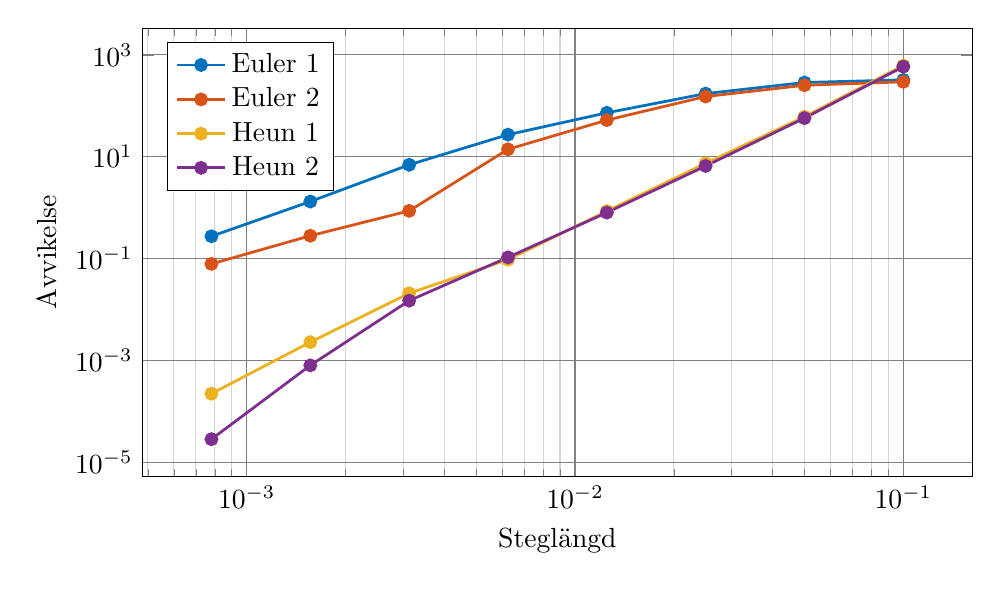
\begin{tikzpicture}
\definecolor{clr0}{RGB}{0, 114, 189}
\definecolor{clr1}{RGB}{217, 83, 25}
\definecolor{clr2}{RGB}{237, 177, 32}
\definecolor{clr3}{RGB}{126, 47, 142}
\definecolor{clr4}{RGB}{119, 172, 48}
\definecolor{clr5}{RGB}{77, 190, 238}
\definecolor{clr6}{RGB}{162, 20, 47}
\begin{axis}[xmode=log,ymode=log,xlabel=Steglängd,ylabel=Avvikelse,width=\textwidth,height=0.6\textwidth,grid=both,minor grid style={draw=gray!33},major grid style={draw=gray},legend pos=north west,]
\addplot[line width=1pt,mark=*,color=clr0] table {
0.1 321.82499235663323
0.05 285.9143478312979
0.025 173.1252401592812
0.0125 72.58472401797417
0.00625 27.039898437326467
0.003125 6.924256503578425
0.0015625 1.3152663350131242
0.00078125 0.27292808350176817
};
\addlegendentry{Euler 1}
\addplot[line width=1pt,mark=*,color=clr1] table {
0.1 295.06670716290256
0.05 252.70977266692853
0.025 151.707765694578
0.0125 52.155224699794864
0.00625 13.952449282368997
0.003125 0.8616735470734886
0.0015625 0.27991151496299177
0.00078125 0.07833790850101363
};
\addlegendentry{Euler 2}
\addplot[line width=1pt,mark=*,color=clr2] table {
0.1 614.4676360719413
0.05 61.01442185189324
0.025 7.398806649002021
0.0125 0.8524107569016619
0.00625 0.09493098117015264
0.003125 0.020771524304823555
0.0015625 0.0022768700212401627
0.00078125 0.00022120469112625954
};
\addlegendentry{Heun 1}
\addplot[line width=1pt,mark=*,color=clr3] table {
0.1 585.6039570794713
0.05 57.15205886985191
0.025 6.5556784468892895
0.0125 0.7972843832850447
0.00625 0.1054098706913994
0.003125 0.014858676340594089
0.0015625 0.0007968407115073739
0.00078125 2.8269099477729043e-05
};
\addlegendentry{Heun 2}
\end{axis}
\end{tikzpicture}
        \caption{Inhomogen}
    \end{subfigure}

    \caption{Avvikelsen i system 8 för de olika funktionerna.}
    \label{fig:diagram_sys_8_errors}
\end{figure}

\clearpage

\subsection{Skillnad mellan Eulers metod och Heuns metod}
Andelsskillnaden mellan Euler och Heuns metod för alla systemen finnes i figur \ref{fig:diff_euler_heun}. Andelsskillnaden räknades ut genom att dividera medelvärdet av avvikelsen i Heuns i de två funktionerna metod med medelvärdet av avvikelsen Eulers metod i de två funktionerna:
\begin{equation}
    \frac{\frac{1}{2}(H_1+H_2)}{\frac{1}{2}(E_1+E_2)}=\frac{H_1+H_2}{E_1+E_2}
\end{equation} där \(H_n\) är avvikelsen i Heuns metod för ekvation \(n\) och \(E_n\) är avvikelsen i Heuns metod för ekvation \(n\). Varje linje är således ett system. För system 5-8 användes de inhomogena ekvationerna.

\begin{figure}[h!]
    \centering
    % Automatically generated code. github.com/ohman-emil/GA
\begin{tikzpicture}
\definecolor{clr0}{RGB}{0, 114, 189}
\definecolor{clr1}{RGB}{217, 83, 25}
\definecolor{clr2}{RGB}{237, 177, 32}
\definecolor{clr3}{RGB}{126, 47, 142}
\definecolor{clr4}{RGB}{119, 172, 48}
\definecolor{clr5}{RGB}{77, 190, 238}
\definecolor{clr6}{RGB}{162, 20, 47}
\definecolor{clr7}{RGB}{120, 120, 120}
\begin{axis}[xmode=log,ymode=log,xlabel=Steglängd,ylabel=Andelsskillnad,width=\textwidth,height=0.6\textwidth,grid=both,minor grid style={draw=gray!33},major grid style={draw=gray},legend pos=north west,legend columns=2,legend style={column sep=1.5ex},]
\addplot[line width=1pt,mark=*,color=clr0] table {
0.05 0.009922132143560405
0.025 0.0021120936100561096
0.0125 0.0004910318982839835
0.00625 0.00013559417714800956
0.003125 4.6445057178022354e-05
0.0015625 1.8774865709994553e-05
0.00078125 8.389478398387147e-06
0.000390625 3.959426664809693e-06
};
\addlegendentry{\hspace{{-1.25ex}}1}
\addplot[line width=1pt,mark=*,color=clr1] table {
0.05 0.050556538000862856
0.025 0.011309724991604549
0.0125 0.003143559731117221
0.00625 0.0011082350541449845
0.003125 0.0004596729075744131
0.0015625 0.00020882175336479994
0.00078125 9.947206455073632e-05
0.000390625 4.853995819442036e-05
};
\addlegendentry{\hspace{{-1.25ex}}2}
\addplot[line width=1pt,mark=*,color=clr2] table {
0.05 0.8997347426829206
0.025 0.31871089445231204
0.0125 0.08241541799367944
0.00625 0.02089211829054193
0.003125 0.005957330967845668
0.0015625 0.002053549644721591
0.00078125 0.0008299256522753324
0.000390625 0.0003704619930878614
};
\addlegendentry{\hspace{{-1.25ex}}3}
\addplot[line width=1pt,mark=*,color=clr3] table {
0.05 0.07915464254958364
0.025 0.02407563602670065
0.0125 0.009016873956865498
0.00625 0.003857633489856828
0.003125 0.0017788131010753126
0.0015625 0.0008534628913396609
0.00078125 0.0004179380765124746
0.000390625 0.00020679462427746715
};
\addlegendentry{\hspace{{-1.25ex}}4}
\addplot[line width=1pt,mark=*,color=clr4] table {
0.05 1.0017607067757557
0.025 0.2902491985666515
0.0125 0.11907813435558601
0.00625 0.055115360286435655
0.003125 0.026652579336928033
0.0015625 0.01312225875935059
0.00078125 0.006512757406788265
0.000390625 0.0032446073083321845
};
\addlegendentry{\hspace{{-1.25ex}}5}
\addplot[line width=1pt,mark=*,color=clr5] table {
0.05 0.03325561692775567
0.025 0.009119215683286136
0.0125 0.002397598302085827
0.00625 0.0006451716895103625
0.003125 0.0001979905958505815
0.0015625 7.2169114617838e-05
0.00078125 3.0126684069708457e-05
0.000390625 1.367930984236576e-05
};
\addlegendentry{\hspace{{-1.25ex}}6}
\addplot[line width=1pt,mark=*,color=clr6] table {
0.05 0.023562190824896804
0.025 0.0064320678229022165
0.0125 0.001688452301188555
0.00625 0.00046155787496610464
0.003125 0.00014538582594452948
0.0015625 5.344090525366828e-05
0.00078125 2.2247340946575404e-05
0.000390625 1.005800498946761e-05
};
\addlegendentry{\hspace{{-1.25ex}}7}
\addplot[line width=1pt,mark=*,color=clr7] table {
0.05 0.6015372851752119
0.025 0.12376697511034081
0.0125 0.030890946907541662
0.00625 0.00814302779416801
0.003125 0.0025015142804039967
0.0015625 0.0009238237455104076
0.00078125 0.0003904453891323726
0.000390625 0.0001787204332109305
};
\addlegendentry{\hspace{{-1.25ex}}8}
\end{axis}
\end{tikzpicture}
    \caption{Andelsskillnaden mellan Eulers metod och Heuns metod.}
    \label{fig:diff_euler_heun}
\end{figure}
